\documentclass[aspectratio=169]{beamer}

\setbeamersize{text margin left=5mm, text margin right=5mm}

\defbeamertemplate{headline}{my header}{%
\vskip1pt%
\makebox[0pt][l]{\,\insertshortauthor}%
\hspace*{\fill}\insertshorttitle/\insertshortsubtitle\hspace*{\fill}%
\llap{\insertpagenumber/\insertpresentationendpage\,}
}
\setbeamertemplate{headline}[my header]

\let\olditem\item
\renewcommand{\item}{\setlength{\itemsep}{\fill}\olditem}

\usepackage{bm}
\usepackage{graphicx}
\usepackage{caption}
\usepackage{soul}
\usepackage{tkz-euclide}
\usetikzlibrary{calc}
\usepackage[]{algorithm2e}
\usepackage{changepage}
\usepackage{amssymb}
\usepackage{xcolor}
\usepackage{mathtools}
\usepackage{tcolorbox}
\usepackage{tikz}
\usepackage{tikz-3dplot}
\usepackage{tkz-euclide}
\usepackage{pgfplots}
\pgfplotsset{width=5cm,compat=1.3}
\usepackage{circuitikz}
\usepackage{mleftright}
% \usepackage{algorithm,algorithmic}
\usetikzlibrary{arrows.meta, decorations.pathreplacing, positioning, shapes.geometric}
\usetikzlibrary{arrows}

\usepackage{pgfplots}
\usetikzlibrary{plotmarks}
\pgfplotsset{width=7cm,compat=1.8}
\pgfplotsset{compat=1.17}

\usetikzlibrary{positioning}
% \usepackage[math]{cellspace}
% \cellspacetoplimit 4pt
% \cellspacebottomlimit 4pt
%\usetikzlibrary{arrows.meta}
% sqare of half axes
\newcommand{\asa}{3}
\newcommand{\bsa}{1}
\newcommand{\csa}{0.25}
% view angle
\tdplotsetmaincoords{70}{135}


%% Fonts
\usefonttheme{professionalfonts}
\usefonttheme{serif}

\DeclareCaptionLabelFormat{blank}{}
\captionsetup[figure]{labelformat=blank}

%% Math definitions
\def\mf{\ensuremath\mathbf}
\def\mb{\ensuremath\mathbb}
\def\mc{\ensuremath\mathcal}
\def\lp{\ensuremath\left(}
\def\rp{\ensuremath\right)}
\def\lv{\ensuremath\left\lvert}
\def\rv{\ensuremath\right\rvert}
\def\lV{\ensuremath\left\lVert}
\def\rV{\ensuremath\right\rVert}
\def\lc{\ensuremath\left\{}
\def\rc{\ensuremath\right\}}
\def\ls{\ensuremath\left[}
\def\rs{\ensuremath\right]}
\def\bmx{\ensuremath\begin{bmatrix*}[r]}
\def\emx{\ensuremath\end{bmatrix*}}
\def\bmxc{\ensuremath\begin{bmatrix*}[c]}
\def\R{\ensuremath\mb{R}}
\def\t{\lp t\rp}
\def\k{\ls k\rs}

\newcommand{\demoex}[2]{\onslide<#1->\begin{color}{black!60} #2 \end{color}}
\newcommand{\demoexc}[3]{\onslide<#1->\begin{color}{#2} #3 \end{color}}
\newcommand{\anim}[3]{\onslide<#1->{\begin{color}{#2!60} #3 \end{color}}}
\newcommand{\ct}[1]{\lp #1\rp}
\newcommand{\dt}[1]{\ls #1\rs}
\newcommand{\cols}[2]{\begin{columns}[#1] #2 \end{columns}}
\newcommand{\col}[2]{\begin{column}{#1} #2 \end{column}}

%% Mycolors
\definecolor{myred}{RGB}{192,0,0}
\definecolor{mygray}{RGB}{100,100,100}

%% Custom beamer color
\setbeamercolor{title}{fg=myred}
\setbeamercolor{subtitle}{fg=myred}
\setbeamerfont{title}{series=\bfseries}
% \setbeamercolor{frametitle}{bg=myred, fg=white}
\setbeamercolor{frametitle}{bg=mygray!10!, fg=myred}
\setbeamerfont{frametitle}{series=\bfseries}
\setbeamercolor{item}{fg=mygray}
\setbeamercolor{title in head/foot}{fg=myred}

% Move header to footer
\setbeamertemplate{headline}{}
\setbeamertemplate{footline}{
  \begin{beamercolorbox}[wd=\paperwidth,ht=2.25ex,dp=1ex,center]{footline}
    \inserttitle\hfill\insertauthor\hfill\insertdate\hfill\insertframenumber{}
  \end{beamercolorbox}
}

\pgfplotsset{
colormap={whitered}{color(0cm)=(white); color(1cm)=(orange!75!red)}
}


\title{Applied Linear Algebra in Data Analysis}

% A subtitle is optional and this may be deleted
\subtitle{Introduction to Constrained Optimization}

\author{Sivakumar Balasubramanian}
% - Give the names in the same order as the appear in the paper.
% - Use the \inst{?} command only if the authors have different
%   affiliation.

\institute[Christian Medical College] % (optional, but mostly needed)
{
  \inst{}%
  Department of Bioengineering\\
  Christian Medical College, Bagayam\\
  Vellore 632002
}
% - Use the \inst command only if there are several affiliations.
% - Keep it simple, no one is interested in your street address.

\date{}
% - Either use conference name or its abbreviation.
% - Not really informative to the audience, more for people (including
%   yourself) who are reading the slides online

\subject{Lecture notes on ALADA}
% This is only inserted into the PDF information catalog. Can be left
% out. 

% If you have a file called "university-logo-filename.xxx", where xxx
% is a graphic format that can be processed by latex or pdflatex,
% resp., then you can add a logo as follows:

% \pgfdeclareimage[height=0.5cm]{university-logo}{university-logo-filename}
% \logo{\pgfuseimage{university-logo}}

% Delete this, if you do not want the table of contents to pop up at
% the beginning of each subsection:
\AtBeginSubsection[]
{
  \begin{frame}<beamer>{Outline}
    \tableofcontents[currentsection,currentsubsection]
  \end{frame}
}

% Let's get started
\begin{document}

\pgfplotsset{
  compat=1.8,
  colormap={whitered}{color(0cm)=(white); color(1cm)=(orange!75!red)}
}


\begin{frame}
  \titlepage
\end{frame}


\begin{frame}[t]{Constrained Optimization}
  \begin{itemize}
    \item A general optimization problem can be fomulated as the following,
    \[ \begin{split}
      \text{minimize}
      & \,\,\, f\ct{\mf{x}} \\
      \mathrm{subject \,\, to} & \,\,\, \mf{g}\ct{\mf{x}} \leq \mf{0}, \,\, \mf{g}\ct{\mf{x}} = \bmx g_1\ct{\mf{x}} & g_2\ct{\mf{x}} & \cdots & g_p\ct{\mf{x}}\emx^\top \\
      & \,\,\, \mf{h}\ct{\mf{x}} = \mf{0}, \,\, \mf{h}\ct{\mf{x}} = \bmx h_1\ct{\mf{x}} & h_2\ct{\mf{x}} & \cdots & h_q\ct{\mf{x}}\emx^\top \\
    \end{split} \]
    where, $f\ct{\mf{x}}$ is the \textbf{objective function} and $\mf{g}\ct{\mf{x}}$ represents the set of \textbf{inquality constaints} and $\mf{h}\ct{\mf{x}}$ represents the set of \textbf{equality constraints}.
  \end{itemize}
\end{frame}


\begin{frame}[t]{Constrained Optimization}
  The set of all values of $\mf{x}$ that satisfy the constraints is called the \textbf{feasible set} and is denoted by $\mc{F}$.
  \[ \mc{F} = \lc \mf{x} \in \mb{R}^n \,\,\mid \,\, \mf{g}\ct{\mf{x}} \leq \mf{0}  \, \text{ and } \, \mf{h}\ct{\mf{x}} = \mf{0} \rc \]
  \vspace{0.2cm}

  Whatever the form, with constrained optimization the search for the minimizer of the function $f\ct{\mf{x}}$ is restricted to the feasible set $\mc{F}$.
  \vspace{0.2cm}
  
  \textbf{Feasible direction} - A direction $\mf{d}$ is said to be a feasible direction at the point $\mf{x} \in \mc{F}$ if there exists $\alpha_0 > 0$ such that $\mf{x} + \alpha \mf{d} \in \mc{F}$ for all $\alpha \in [0, \alpha_0]$.
  \vspace{0.2cm}

  The conditions for a point to be a minimizer in the constrained optimization case are different from the unconstrained case.
\end{frame}


\begin{frame}[t]{Constrained Optimization}
  \textbf{First Order Necessary Condition}. Let $\mc{F} \in \R^n$, and let $f: \mc{F} \to \R$ be a differentiable function (at least once). If $\mf{x}^{\star}$ is a local minimizer of the function $f$ over the set $\mc{F}$, then for any feasible direction $\mf{d}$ at the point $\mf{x}^{\star}$, we have,
  \[ \mf{d}^\top \nabla f\ct{\mf{x}^\star} \geq 0 \]

  This above conditions applies for both points at the boundary and interior to the set $\mc{F}$.
  \vspace{0.2cm}

  For interior points, all directions are feasible, and so the above condition becomes,
  \[ \nabla f\ct{\mf{x}^\star} = 0 \]
  which is the same as the unconstrained case.
\end{frame}


\begin{frame}[t]{Constrained Optimization}
  \textbf{Second Order Necessary Condition}. Let $\mc{F} \in \R^n$, and let $f: \mc{F} \to \R$ be a differentiable function (at least twice), $\mf{x}^{\star}$ is a local minimizer of $f$ over $\mc{F}$, and $\mf{d}$ is a feasible direction at $\mf{x}^{\star}$. If $\mf{d}^\top\nabla f\ct{\mf{x}} = 0$, then 
  \[ \mf{d}^\top \mf{H}\ct{\mf{x}^\star}\mf{d} \geq 0 \]
  where $\mf{H}\ct{\mf{x}}$ is the Hessian of $f$ at $\mf{x}$.
  \vspace{0.2cm}
\end{frame}


\begin{frame}[t]{Constrained Optimization: Equality Constraints}
  Consider the following optimization problem with only equality constraints,
  \[ \begin{split}
    \text{minimize}
    & \,\,\, f\ct{\mf{x}} \\
    \mathrm{subject \,\, to} & \,\,\, \mf{h}\ct{\mf{x}} = \mf{0} \\
  \end{split} \]
  where, $\mf{h}\ct{\mf{x}} = \bmx h_1\ct{\mf{x}} & h_2\ct{\mf{x}} & \cdots & h_q\ct{\mf{x}}\emx^\top$, and we assume that each one of these constraint functios is differentiable.
  \vspace{0.2cm}

  The feasible set for this problem is,
  \[ \mc{F} = \lc \mf{x} \in \mb{R}^n \,\,\mid \,\, \mf{h}\ct{\mf{x}} = \mf{0} \rc \]

  Note that the feasiblity set forms a $n - q$ dimensional surface oer manifold in $\R^n$.
\end{frame}


\begin{frame}[t]{Constrained Optimization: Equality Constraints}
  \textbf{Regular point} -- A point $\mf{x}^{\star} \in \mc{F}$ is said to be a regular point if the gradients of the equality constraints are linearly independent at the point $\mf{x}^{\star}$.
  \vspace{0.2cm}
  
  Note that the gradient of the equality constraints is a matrix of size $q \times n$.
  \[ \nabla_{\mf{x}} \mf{h}\ct{\mf{x}} =  \bmx \nabla_{\mf{x}} h_1\ct{\mf{x}} \\ \nabla_{\mf{x}} h_2\ct{\mf{x}} \\ \vdots \\ \nabla_{\mf{x}} h_q\ct{\mf{x}}\emx \in \R^{q \times n} \]
  
  The gradient $\nabla \mf{h}\ct{\mf{x}}$ has full rank at a regular point.

\end{frame}


\begin{frame}[t]{Constrained Optimization: Equality Constraints}
  The \textbf{tangent space} of a surface is the higher dimensional equivalent of a tagent line to a one dimensional curve. 
  \vspace{0.2cm}

  The \textbf{tangent space} at a point $\mf{x}^\star \in \mc{F}$ is defined as the following set,
  \[ T\ct{\mf{x}^\star} = \lc \mf{y} \in \R^n \, \mid \, \nabla \mf{h}\ct{\mf{x}} \mf{y} = \mf{0} \rc = \mc{N}\ct{\nabla \mf{h}\ct{\mf{x}}} \]
  
  The \textbf{tangent plane} at the point $\mf{x}^\star$ on the surface $\mc{F}$ is defined as,
  \[ TP\ct{\mf{x}^\star} = T\ct{\mf{x}^\star} + \mf{x}^\star = \lc \mf{x} + \mf{x}^\star \, \mid \, \mf{x} \in T\ct{\mf{x}^\star} \rc \]
\end{frame}


\begin{frame}[t]{Constrained Optimization: Equality Constraints}
  The \textbf{normal space} of a surface is the orthogonal complement of the tangent space.  
  \vspace{0.2cm}

  The \textbf{normal space} at a point $\mf{x}^\star \in \mc{F}$ is defined as the following set,
  \[ N\ct{\mf{x}^\star} = \lc \nabla \mf{h}\ct{\mf{x}}^\top \mf{y} \, \mid \, \mf{y} \in \R^q \rc = \mc{R}\ct{\nabla \mf{h}\ct{\mf{x}}^\top } \]
  
  The \textbf{normal plane} at the point $\mf{x}^\star$ on the surface $\mc{F}$ is defined as,
  \[ NP\ct{\mf{x}^\star} = N\ct{\mf{x}^\star} + \mf{x}^\star = \lc \mf{x} + \mf{x}^\star \, \mid \, \mf{x} \in N\ct{\mf{x}^\star} \rc \]
\end{frame}


\begin{frame}[t]{Constrained Optimization: Equality Constraints}
  \textbf{Lagrange theorem}: Let $\mf{x}^\star$ be a local minimizer (or maximizer) of the function $f: \R^n \to \R$, subject to $\mf{h}\ct{\mf{x}} = \mf{0}$, $\mf{h}: \R^n \to \R^q$, $q \leq n$. Assume that $\mf{x}^\star$ is a regular point of the equality constraints. Then there exists a vector $\bm{\lambda}^\star \in \R^q$ such that,
  \[ \nabla f\ct{\mf{x}^\star} + \nabla \mf{h}\ct{\mf{x}^\star}^\top \bm{\lambda}^\star = \mf{0} \]
  where, $\bm{\lambda}^\star$ is called the \textbf{Lagrange multiplier vector}.
  \vspace{0.2cm}

  This theorem states that extremum of this constrained optimization problem occurs when the gradient of $f$ is in the normal space of the surface $\mc{F}$, i.e. $\nabla f\ct{\mf{x}}$ is a linear combination of the gradients of the individual equality constraints $\nabla h_i\ct{\mf{x}}$, $1 \leq i \leq q$.
  \vspace{0.2cm}

  This is also equivalent to saying $\nabla f\ct{\mf{x}} \in T\ct{\mf{x}}^\perp$ or $\nabla f\ct{\mf{x}} \in N\ct{\mf{x}}$
\end{frame}


\begin{frame}[t]{Constrained Optimization: Equality Constraints}
  It is convenient to introduce the \textbf{Lagrange function}: $l: \R^n \times \R^q \to \R$, 
  \[ l\ct{\mf{x}, \bm{\lambda}} = f\ct{\mf{x}} + \bm{\lambda}^\top\mf{f}\ct{\mf{x}} \]
  The Lagrange condition for $\mf{x}^\star$ to be a local minimizer is the following,
  \[ \nabla l\ct{\mf{x}^\star, \bm{\lambda}^\star} = \mf{0} \]
  for some $\bm{\lambda}^\star$, where the gradient is with respect to the combined argument $\bmx \mf{x}^\top & \bm{\lambda}^\top\emx$.
  \vspace{0.2cm}
  This is equivalent to the first order necessary condition for the unconstrained optimization problem with respect to $\bmx \mf{x}^\top & \bm{\lambda}^\top\emx$.
  \vspace{0.2cm}
  This condition is necessary but not sufficient.
\end{frame}


\begin{frame}[t]{Constrained Optimization: Equality Constraints}
  Let $f$ and $\mf{h}$ be both twice continuously differentiable,
  \[ \begin{split}
    l\ct{\mf{x}, \bm{\lambda}} &= f\ct{\mf{x}} + \bm{\lambda}^\top\mf{f}\ct{\mf{x}} \\
     &= f\ct{\mf{x}} + \lambda_1 h_1\ct{\mf{x}} + \lambda_2 h_2\ct{\mf{x}} + \cdots + \lambda_q h_q\ct{\mf{x}}
  \end{split} \]
  Taking the Hessian on both sides,
  \[ \mf{H}_{l}\ct{\mf{x}} = \mf{H}_f\ct{\mf{x}} + \sum_{i=1}^q \lambda_i \mf{H}_{h_i}\ct{\mf{x}} \]
  where $\mf{H}_l$ is the Hessian of $l\ct{\mf{x}, \bm{\lambda}}$ with respect to $\mf{x}$, and $\mf{H}_{h_i}$ is the Hessian of the function $h_i\ct{\mf{x}}$ with respect to $\mf{x}$. 
\end{frame}


\begin{frame}[t]{Constrained Optimization: Equality Constraints}
  \textbf{Second Order Necessary Condition}. Let $\mf{x}^\star$ be a local minimizer of $f$ subject to the equality constraints $\mf{h}\ct{\mf{x}} = \mf{0}$, $\mf{h}: \R^n \to \R^q$, $q \leq n$, and $f, \mf{h}$ are twice differentiable, and $\mf{x}^\star$ is a regular point. Then, there exists a vector $\bm{\lambda}^\star \in \R^q$ such that,
  \begin{enumerate}
    \item $\nabla f\ct{\mf{x}^\star} + {\bm{\lambda}^\star}^\top \nabla \mf{h}\ct{\mf{x}} = \mf{0}$
    \item For all $\mf{y} \in T\ct{\mf{x}^\star}$, we have $\mf{y}^\top \mf{L}\ct{\mf{x}^\star, \bm{\lambda}^\star}\mf{y} \geq 0$.
  \end{enumerate}
  \vspace{1cm}

  \textbf{Second Order Sufficient Condition}. $\mf{x}^\star$ is strict local minimizer of $f$ subject to the equality constraints $\mf{h}\ct{\mf{x}} = \mf{0}$, $\mf{h}: \R^n \to \R^q$,
  \begin{enumerate}
    \item $\nabla f\ct{\mf{x}^\star} + {\bm{\lambda}^\star}^\top \nabla \mf{h}\ct{\mf{x}} = \mf{0}$
    \item For all $\mf{y} \in T\ct{\mf{x}^\star}$, we have $\mf{y}^\top \mf{L}\ct{\mf{x}^\star, \bm{\lambda}^\star}\mf{y} > 0$.
  \end{enumerate}
\end{frame}


\begin{frame}[t]{Constrained Optimization: Inequality Constraints}
  \[ \begin{split}
    \text{minimize}
    & \,\,\, f\ct{\mf{x}} \\
    \mathrm{subject \,\, to} & \,\,\, \mf{g}\ct{\mf{x}} \leq \mf{0}, \,\, \mf{g}\ct{\mf{x}} = \bmx g_1\ct{\mf{x}} & g_2\ct{\mf{x}} & \cdots & g_p\ct{\mf{x}}\emx^\top \\
    & \,\,\, \mf{h}\ct{\mf{x}} = \mf{0}, \,\, \mf{h}\ct{\mf{x}} = \bmx h_1\ct{\mf{x}} & h_2\ct{\mf{x}} & \cdots & h_q\ct{\mf{x}}\emx^\top \\
  \end{split} \]
  where, $f\ct{\mf{x}}$ is the \textbf{objective function} and $\mf{g}\ct{\mf{x}}$ represents the set of \textbf{inquality constaints} and $\mf{h}\ct{\mf{x}}$ represents the set of \textbf{equality constraints}.
  \vspace{0.25cm}

  An inequality constraint $g_i\ct{\mf{x}} \leq 0$ is said to be \textbf{active} at a point $\mf{x}^\star$ if $g_i\ct{\mf{x}^\star} = 0$. It is \textbf{inactive} at $\mf{x}^\star$ if $g_i\ct{\mf{x}^\star} < 0$.
\end{frame}


\begin{frame}[t]{Constrained Optimization: Inequality Constraints}
  \textbf{Regular point} Let the point $\mf{x}^\star$ satisfy $\mf{h}\ct{\mf{x}^\star} = \mf{0}$, $\mf{g}\ct{\mf{x}^\star} \leq \mf{0}$, and let $J\ct{\mf{x}^\star}$ be the index set of active inquality constraints,
  \[ J\ct{\mf{x}^\star} = \lc j \, \mid \, g_j\ct{\mf{x}^\star} = 0 \rc \]
  We say the point $\mf{x}^\star$ is a \textbf{regular point} if the following vectors form a linearly independent set.
  \[ \nabla h_i\ct{\mf{x}^\star}, \, \nabla g_j\ct{\mf{x}^\star}, \,\, 1 \leq i \leq q, \, j \in J\ct{\mf{x}^\star} \]
\end{frame}


\begin{frame}[t]{Constrained Optimization: Inequality Constraints}
  \textbf{Karush-Kuhn-Tucker Theorem}. Let $f, \mf{h}, \mf{g}$ be differentiable at least once, and let $\mf{x}^\star$ be a regular point and a local minimizer of the problem. Then, there exists $\bm{\lambda}^\star \in \R^q$ and $\bm{\mu}^\star \in \R^p$ such that,
  \begin{enumerate}
    \item $\bm{\mu}^\star \geq 0$
    \item $\nabla f\ct{\mf{x}^\star} + \nabla \mf{h}\ct{\mf{x}^\star}^\top {\bm{\lambda}^\star} + \nabla \mf{g}\ct{\mf{x}^\star}^\top {\bm{\mu}^\star} = \mf{0}$
    \item ${\bm{\mu}^\star}^\top \mf{g}\ct{\mf{x}^\star} = 0$
  \end{enumerate}
  \vspace{1cm}

  The vector $\bm{\lambda}^\star$ is called the \textbf{Lagrange multiplier vector} and $\bm{\mu}^\star$ is called the \textbf{Karush-Kuhn-Tucker (KKT) multiplier vector}.
  \vfill
\end{frame}


\begin{frame}[t]{Constrained Optimization: Inequality Constraints}
  \begin{figure}
    \centering
    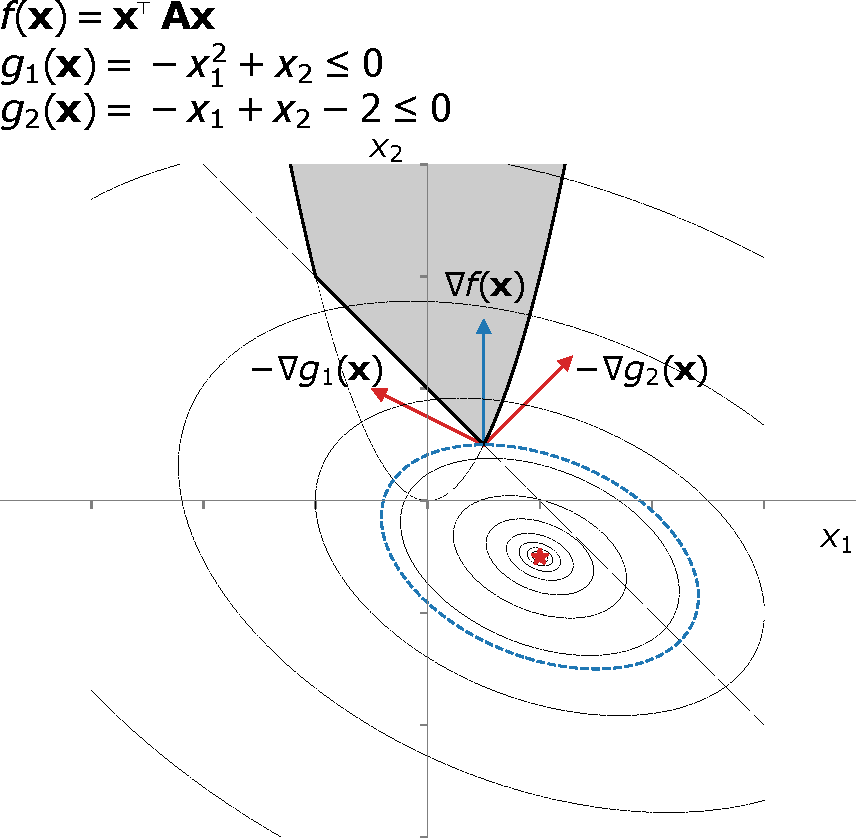
\includegraphics[width=0.45\textwidth]{figs/ineq_const.pdf}
  \end{figure}
\end{frame}


\begin{frame}[t]{Constrained Optimization: Inequality Constraints}
  \textbf{Tangent space}: The tangent space at a point $\mf{x}^\star$ is defined as,
  \[ T\ct{\mf{x}^\star} = \lc \mf{y} \in \R^n \, \mid \, \nabla \mf{h}\ct{\mf{x}^\star} \mf{y} = \mf{0}, \nabla g_j\ct{\mf{x}^\star}^\top \mf{y} = 0, \,\, j \in J\ct{\mf{x}^\star} \rc \]
  \vspace{0.25cm}

  \textbf{Second order necessary condition.} Let $\mf{x}^\star$ be a local minimizer of $f\ct{\mf{x}}$ subject to $\mf{h}\ct{\mf{x}^\star} = \mf{0}$ and $\mf{g}\ct{\mf{x}} \leq \mf{0}$. Let $f, \mf{h}, \mf{g}$ be at least twice differentiableThen, there exists $\bm{\lambda}^\star \in \R^q$ and $\bm{\mu}^\star \in \R^p$ such that, 
  \begin{enumerate}
    \item $\nabla f\ct{\mf{x}^\star} + \nabla \mf{h}\ct{\mf{x}^\star}^\top {\bm{\lambda}^\star} + \nabla \mf{g}\ct{\mf{x}^\star}^\top {\bm{\mu}^\star} = \mf{0}$
    \item For all $\mf{y} \in T\ct{\mf{x}^\star}$, we have $\mf{y}^\top \mf{H}\ct{\mf{x}^\star, \bm{\lambda}^\star, \bm{\mu}^\star}\mf{y} \geq 0$.
  \end{enumerate}
  where,
  \[ \mf{H}\ct{\mf{x}} = \mf{H}_f\ct{\mf{x}} + \sum_{i=1}^p \mu_i \mf{H}_{g_i}\ct{\mf{x}} + \sum_{i=1}^q \lambda_i \mf{H}_{h_i}\ct{\mf{x}} \]
\end{frame}


\begin{frame}[t]{Constrained Optimization: Inequality Constraints}
  \textbf{Second order sufficient condition.} Let $\mf{x}^\star$ be a local minimizer of $f\ct{\mf{x}}$ subject to $\mf{h}\ct{\mf{x}^\star} = \mf{0}$ and $\mf{g}\ct{\mf{x}} \leq \mf{0}$. Let $f, \mf{h}, \mf{g}$ be at least twice differentiableThen, there exists $\bm{\lambda}^\star \in \R^q$ and $\bm{\mu}^\star \in \R^p$ such that, 
  \begin{enumerate}
    \item $\nabla f\ct{\mf{x}^\star} + \nabla \mf{h}\ct{\mf{x}^\star}^\top {\bm{\lambda}^\star} + \nabla \mf{g}\ct{\mf{x}^\star}^\top {\bm{\mu}^\star} = \mf{0}$
    \item For all $\mf{y} \in \tilde{T}\ct{\mf{x}^\star}$, we have $\mf{y}^\top \mf{H}\ct{\mf{x}^\star, \bm{\lambda}^\star, \bm{\mu}^\star}\mf{y} \geq 0$.
  \end{enumerate}
  where,
  \[ \mf{H}\ct{\mf{x}} = \mf{H}_f\ct{\mf{x}} + \sum_{i=1}^p \mu_i \mf{H}_{g_i}\ct{\mf{x}} + \sum_{i=1}^q \lambda_i \mf{H}_{h_i}\ct{\mf{x}} \]
  and,
  \[ \tilde{T}\ct{\mf{x}^\star} = \lc \rc \]
  \vspace{0.5cm}

  $\mf{x}^\star$ is a strict local minimizer of $f\ct{\mf{x}}$ subject to $\mf{h}\ct{x} = \mf{0}$ and $\mf{g}\ct{\mf{x}} \leq \mf{0}$.
\end{frame}

\end{document}